\section{Thermal Analysis}

As seen from MOSFET and Diode loss calculation, there is required heat sink for MOSFET and Diode to protect components from higher temperature. Diode and MOSFET have typical working temperature. Temperature of these components should be between temperature limitations. Losses of the system is dissipated as heat. This heat can damage our components. There is required electric circuit equivalent of thermal design to do better thermal analysis. Required thermal resistance values can be found from data sheets of diode MOSFET and heat sinks. Electric circuit equivalent of thermal analysis is given Figure \ref{fig:wo-hs}.

\begin{figure}[H]
\begin{center}
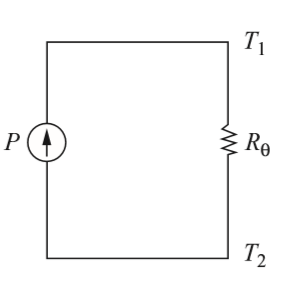
\includegraphics[width=0.4\textwidth]{figures/wo-hs.PNG}
\caption{An Electric Circuit Equivalent of Thermal Analysis without Heat Sink}
\label{fig:wo-hs}
\end{center}
\end{figure}

As seen from Figure \ref{fig:wo-hs}, $R_{\theta}$ is the sum of junction to case thermal resistance and case to ambient thermal resistance which are, $R_{th,j-c}$ and $R_{th,c-a}$. 
$$R_{\theta} = \frac{T_1 - T_2 }{P_{loss}}$$

Equivalent circuit of system is changed after heat sink addition. When there is lower thermal resistance, it means there is lower temperature increases. At Figure \ref{fig:w-hs}, equivalent circuit of thermal analysis with heat sink is given. 

\begin{figure}[H]
\begin{center}
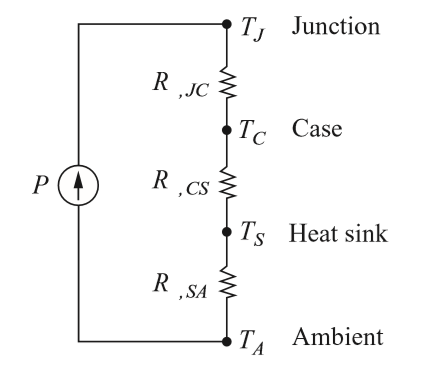
\includegraphics[width=0.5\textwidth]{figures/with hs.PNG}
\caption{An Electric Circuit Equivalent of Thermal Analysis with Heat Sink}
\label{fig:w-hs}
\end{center}
\end{figure}

$R_{,CS}$ and $R_{,SA}$ is  given by manufacturer of the heat sink. Sum of these two thermal resistance is important for thermal analysis and can be found from heat sink data sheet. Thermal design of the converter will be done according to these equivalent circuits.

\subsection{MOSFET Heat Sink Selection}

As seen from efficiency section, there is more power losses on the MOSFET when the input voltage is higher. So, thermal design of the system will be done according to minimum input voltage value. System should be designated for maximum power loss condition. Working temperature of the MOSFET is -55 to 150 \degree C . 125 \degree C is selected to have better thermal design. Maximum limitation of the system is reduced. There should be unexpected situations, that is why 125\degree C is better for limitation. Required parameters and measurements are given below for thermal analysis. Ambient temperature is taken as 25\degree C.

$$R_{thj-c}\ =\ 3.6\ \degree C / W$$
$$R_{thc-amb}\ =\ 62.5\ \degree C / W$$
$$P_{FET} = P_{CON}+P{SW} = 7.0225+0.11 = 7.1325\ W$$

Without heat sink, to reach 125\degree C, required power calculation is given below;

\begin{align}
    P_{Thermal} = \frac{T_1 - T_2}{R_\theta} = \frac{125-25}{62.5+3.6} = 1.513\ W \\
\end{align}

1.513 W is enough to damage our MOSFET. There is power loss more than 1.513 W which is 7.1325 W. To protect our MOSFET, there is required heat sink which will reduce to case to ambient thermal resistance. When this thermal resistance is reduced, there will be less temperature increases under same power loss. Required heat sink thermal resistance calculation is given below;

\begin{align}
    P_{loss} = 7.1325\ W \\
    P_{loss} = \frac{T_1 - T_2 }{R_{final}}\\
    R_{final} = \frac{100}{7.1325} = 14\ \degree C/W
    R_{heat sink} = R_{final} - R_{thj-c} = 14-3.6 = 10.4\ \degree C/W\\
\end{align}

According to calculations, thermal resistance of the heat sink should be lower than 10.4 \degree C/W. When the cost and thermal analysis is done, Assmann WSW Components, V5220L heat sink is chosen. Price of the heat sink is 0.8 \$. 
$$R_{heat sink} = 8.0\ \degree C/W $$

Thermal analysis after heat sink ;

\begin{align}
    P_{loss} = 7.1325 W = \frac{T_{final}-T_{amb}}{R_{final}}\\
    7.1325 W = \frac{T_{final}-25}{8+3.6} \\
    T_{final} = (7.1325 \times 11.6 ) + 25 = 107.8\ \degree C 
\end{align}

MOSFET temperature at maximum loss condition is 107. 8 \degree C . Which is lower than limitation temperature.

\subsection{Diode Heat Sink Selection}

As seen from efficiency calculations, diode power losses are similar for different input voltage due to constant output power. Diode current is like output current. Maximum power loss on diode is shown at 24 V input voltage but so close to other cases. Required parameters and measurements are given below for thermal analysis and design. Diode working temperatıre is between -65 to 175 \degree C. 150  \degree C is chosen as limitation for diode temperature to have better thermal design. 

$$R_{thj-c}\ =\ 2\ \degree C / W$$
$$R_{thc-amb}\ =\ 60\ \degree C / W$$
$$P_{diode}  = 5.33\ W$$

Without heat sink, to reach 150\degree C, required power calculation is given below;

\begin{align}
    P_{Thermal} = \frac{T_1 - T_2}{R_\theta} = \frac{150-25}{60+2} = 2.02\ W \\
\end{align}

2.02 W is enough to damage our diode. There is power loss more than 2.02 W which is 5.33 W. To protect our diode, there is required heat sink which will reduce to case to ambient thermal resistance. When this thermal resistance is reduced, there will be less temperature increases under same power loss. Required heat sink thermal resistance calculation is given below;

\begin{align}
    P_{loss} = 5.33\ W \\
    P_{loss} = \frac{T_1 - T_2 }{R_{final}}\\
    R_{final} = \frac{125}{5.33} = 23.45\ \degree C/W
    R_{heat sink} = R_{final} - R_{thj-c} = 23.4-2 = 21.4\ \degree C/W\\
\end{align}

According to calculations, thermal resistance of the heat sink should be lower than 21.4 \degree C/W. When the cost and thermal analysis is done, CUI Devices- HSS-B20-NP-01 heat sink is chosen for thermal design. Price of the heat sink is 0.2 \$. 
$$R_{heat sink} = 16.29\ \degree C/W $$

Thermal analysis after heat sink ;

\begin{align}
    P_{loss} = 5.33 W = \frac{T_{final}-T_{amb}}{R_{final}}\\
    5.33 W = \frac{T_{final}-25}{16.29+2} \\
    T_{final} = (5.33 \times 18.29 ) + 25 = 122.49\ \degree C 
\end{align}

Diode temperature at maximum loss condition is 122.49 \degree C . Which is lower than limitation temperature(150 \degree C).

\newpage